\documentclass{article}

% set font encoding for PDFLaTeX or XeLaTeX
\usepackage{ifxetex}
\ifxetex
  \usepackage{fontspec}
\else
  \usepackage[T1]{fontenc}
  \usepackage[utf8]{inputenc}
  \usepackage{lmodern}
  \usepackage{graphicx}
\fi

% used in maketitle
\title{ \begin{center}
        \includegraphics[width=8cm]{unison.png}
        \end{center}
        \newline
       Reporte de Actividad 4}
\author{Jose "Buma" Burruel Martinez}
\date{21 de Febrero del 2018}

% Enable SageTeX to run SageMath code right inside this LaTeX file.
% documentation: http://mirrors.ctan.org/macros/latex/contrib/sagetex/sagetexpackage.pdf
% \usepackage{sagetex}

\begin{document}

\maketitle{Actividad 4}

\section{Introducción}
El sistema operativo UNIX y sus derivados, como Linux, Ubuntu, macOS, y otros, requieren de una interfaz que permita al Usuario comunicarse con la máquina para decirle a esta qué hacer llamada Interprete de comandos, en este caso llamada SHELL, del cual, exploraremos unos cuantos comandos.

\section{Comandos del SHELL}
En ésta actividad de exploraron ciertos comandos con el SHELL llamado /bin/bash que viene por Default en los sistemas operativos ya mencionados. 
\subsection{cat}
El comando \textit{cat} se utiliza para concatenar, es decir, combinar archivos de texto en un solo display en la terminal.
\subsection{chmod}
El comando \textit{chmod} se utiliza para cambiar los permisos de un archivo cualquiera.
Cada archivo puede llegar a tres tipos de personas, el del usuario local, el de los usuarios del grupo o familia, y el de los usuarios otros, y esos a su vez tienen 3 permisos: Lectura, Editar y Ejecutar; con el \textit{chmod} puedes otrogarle o quitarle esos permisos a cada tipo de persona por medio de un sistema binario que rige esos permisos.
\subsection{echo}
El \textit{echo} simplemente imprime en la terminal una palabra, oración o variable que tú elijas.
\subsection{grep}
Este comando hace un filtro en una palabra u oración que tengas en un archivo y te regresa todas las lineas que se encuentran en los archivos que contienen esa cosa que buscabas.
\subsection{less}
EL comando \textit{less} te permite leer un archivo de texto en la terminal.
\subsection{wc}
Este comando te permite contar cuantas lineas tienen una palabra que buscaste en el archivo. Es como el \textit{grep} pero esta te regresa cuantas son, no la linea en sí.
\subsection{ls}
\textit{ls} solamente te enlista en terminal todos los elementos en la carpeta actual. 
Al agregar \textit{-alg} a la derecha de \textit{ls} te muestra los permisos de cada archivo, de ahí puedes revisar cómo cambiar los permisos con \textit{chmod} .
\subsection{Redireccionadores "|" y ">"}
Estos caracteres redirecciónan variables. Por ejemplo, puedes realizar un \textit{egrep} una palabra de un archivo, o varias palabras o variables, separadas con "|" y enviarlas todas a un archivo completamente nuevo por medio del simbolo ">".

\section{Procedimiento}
Lo que hicimos primeramente fue descargar un script para el SHELL de la terminal de Linux que nos permitía descargar datos de sondeo meteorologico de la Universidad de Wyoming, así como en la actividad pasada. Lo siguiente fue editar dicho Script para poder descargar los datos de los 12 meses del 2017, ya que el Script venía como default la descarga de 5 años.  

\begin{figure}
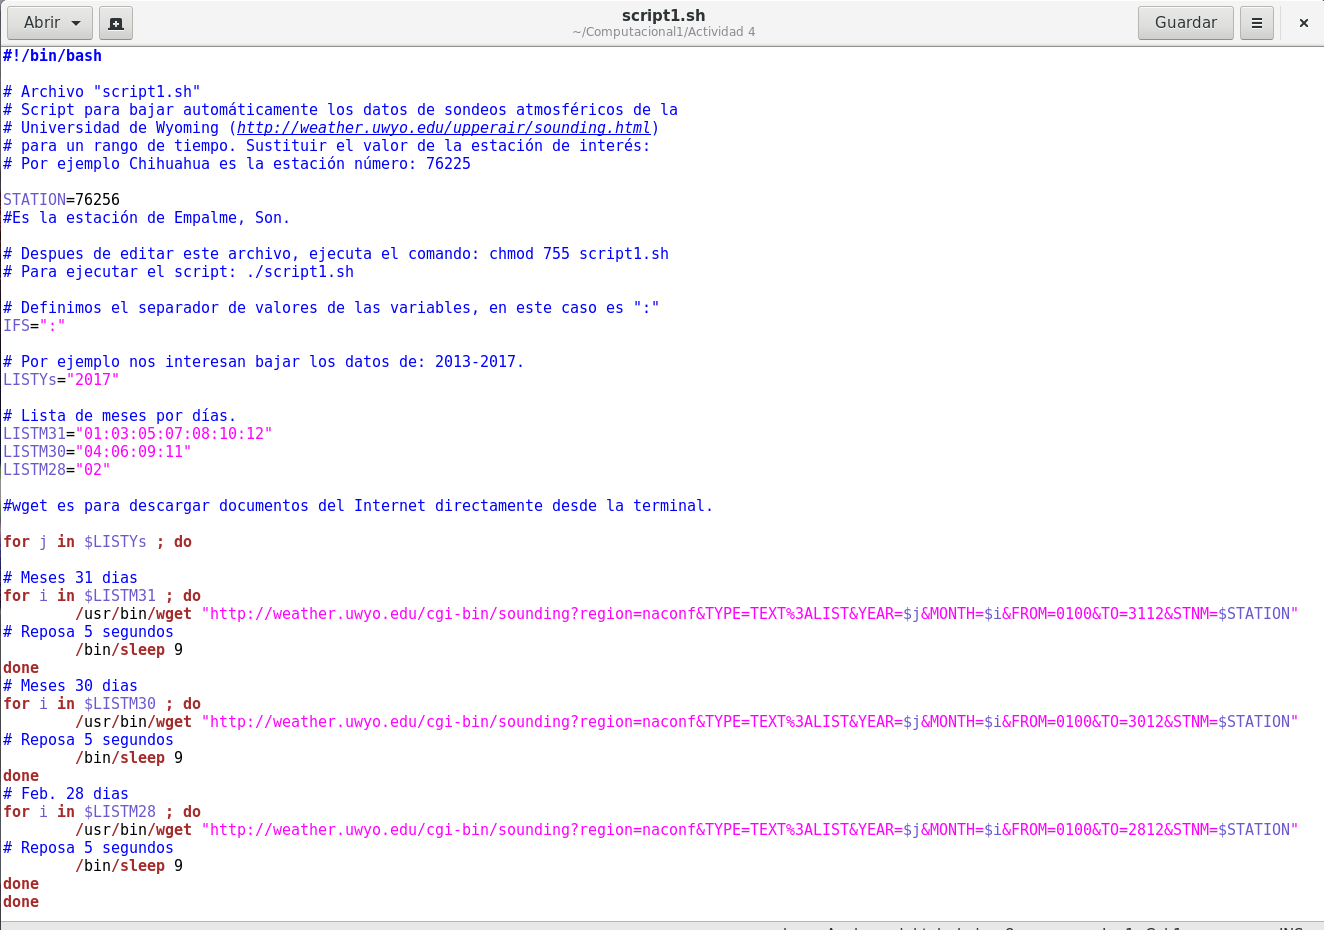
\includegraphics[width=\linewidth]{Script 1.png}
\caption{Script utilizado en la primera parte del ejercicio.}
\end{figure}

Hicimos uso del comando \textit{chmod} para cambiar los permisos y poder correr el programa para poder descargar los datos; acto siguiente, utilizamos los comandos \textit{less y cat} para poder leer los archivos y poder concatenarlos todos en un solo display en la terminal. 
Despues, con un comando \textit{egrep} metimos todos los datos que sí ocuparíamos en un solo archivo llamado \textit{sondeos.txt} con el cual, despues, volveríamos a utilizar un \textit{egrep y redireccionadores "|" y ">"} para sacar solamente la información con la cual se realizaría el futuro análisis de datos. 
Acto siguiente, nosotros mismos crearíamos un Script que automatizara eso ultimo pero para todos los archivos descargados. 

\begin{figure}
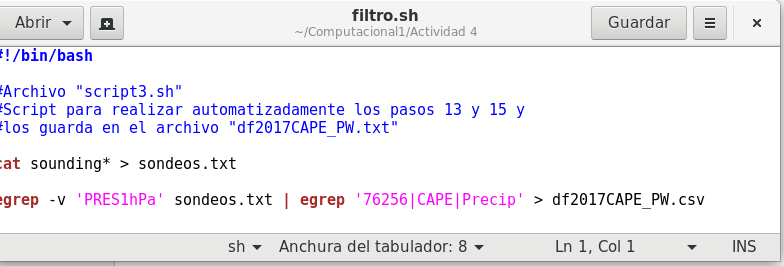
\includegraphics[width=\linewidth]{Filtro.png}
\caption{Script que usamos de filtro.}
\end{figure}

\section{Resultados}
Al seguir cada uno de los pasos proporcionados por el profesor, pudimos realizar la descarga de los datos junto con los archivos \textit{.txt} para su futuro análisis de datos.

\begin{figure}
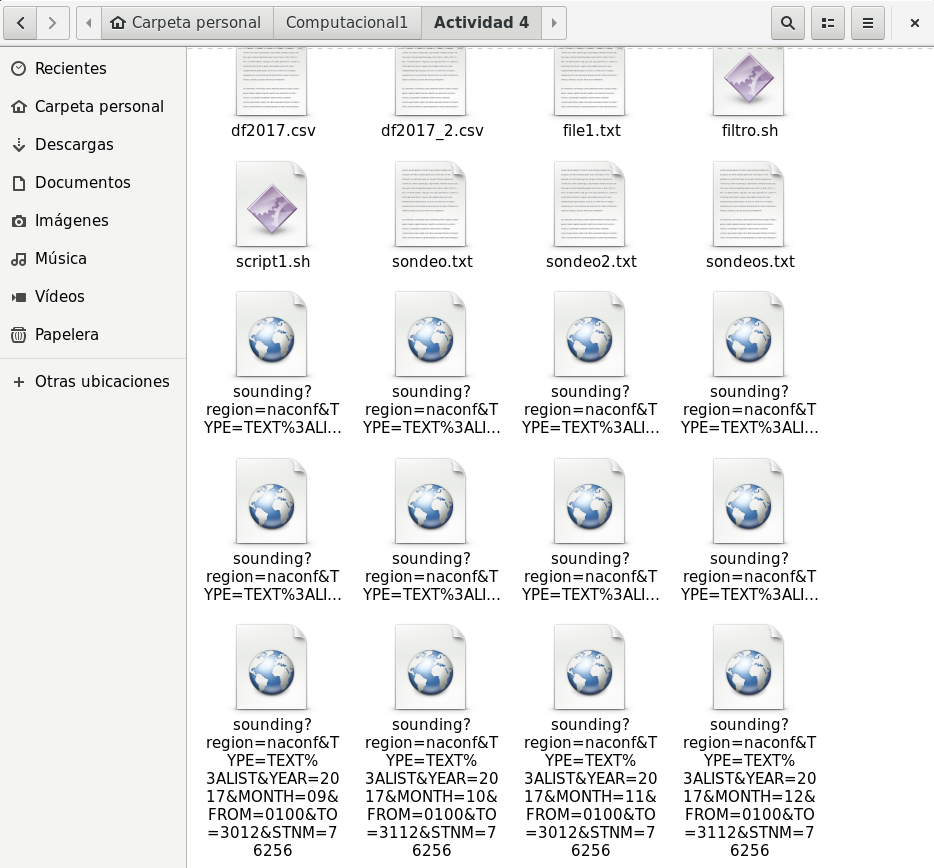
\includegraphics[width=\linewidth]{Sondeos.png}
\caption{Así quedó la carpeta de trabajos, con los archivos de descarga de datos y con los archivos de los datos concatenados para el futuro anlisis.}
\end{figure}

\section{Conclusiones}
Como pudimos apreciar, el SHELL y sus scripts son una manera bastante fácil de hacer que la máquina haga lo que queremos y nos facilita bastante la automatización del procesamiento de este tipo de archivos a otro con el que sí podamos trabajar mucho más fácil.

\newpage

\section{Apéndice}
\subsection{¿Qué fue lo que más te llamó la atención en esta actividad?}
El proceso por el cual descargamos los archivos de la base de datos de la Universidad de Wyoming.
\subsection{¿Qué consideras que aprendiste?}
A utilizar de mejor manera la terminal del sistema operativo de Ubunto y Unix en general.
\subsection{¿Cuáles fueron las cosas que más se te dificultaron?}
Hacer el reporte, como siempre.
\subsection{¿Cómo se podría mejorar en esta actividad?}
Se me hace que así está bien por ahora.
\subsection{¿En general, cómo te sentiste al realizar en esta actividad?}
Bien, siento que aprendí algo muy util en programación científica y el manejo de la terminal.

\end{document}
